Het GMRES algoritme werd ge\"implementeerd als volgt:
\lstinputlisting[
  style      = Matlab-editor,
  basicstyle = \mlttfamily,
]{NMB_gmres.m}

Dit geeft het convergentiegedrag zoals weergegeven in figuur \ref{fig:oef8}  voor verschillende waardes voor \path{alpha}. Hoe groter \path{alpha}, hoe sneller de convergentie. Voor \path{alpha} gelijk aan 1 is er geen convergentie.

\begin{figure*}
	\centering

        \begin{subfigure}[b]{0.475\textwidth}
	\centering
       	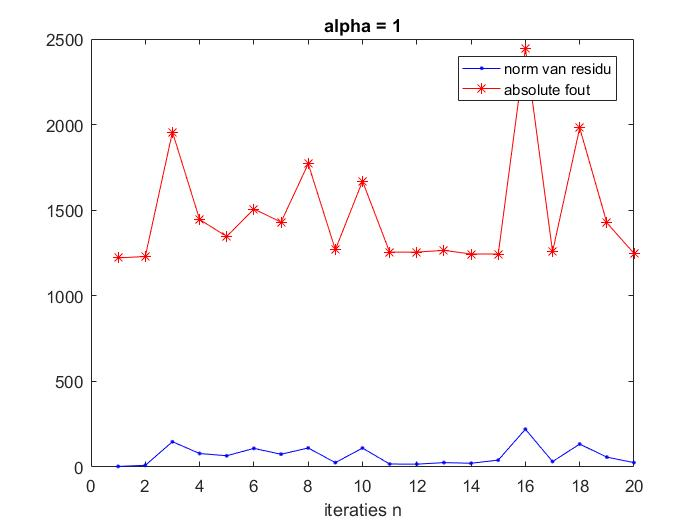
\includegraphics[width=\linewidth]{oef8_1.jpg}
        \caption{{\small alpha = 1}}    
        \label{fig:oef8_1}
        \end{subfigure}

        \hfill

        \begin{subfigure}[b]{0.475\textwidth}
	\centering 
        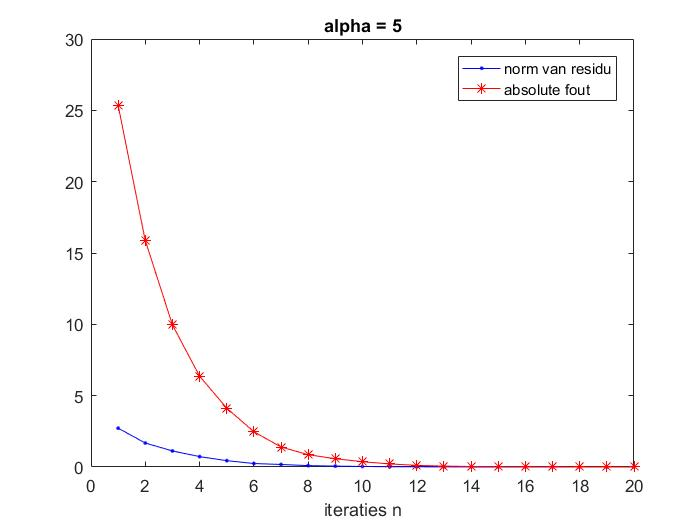
\includegraphics[width=\linewidth]{oef8_5.jpg}
        \caption{{\small alpha = 5}}    
            \label{fig:oef8_5}
        \end{subfigure}

	\bigskip        

        \begin{subfigure}[b]{0.475\textwidth}
	\centering
   	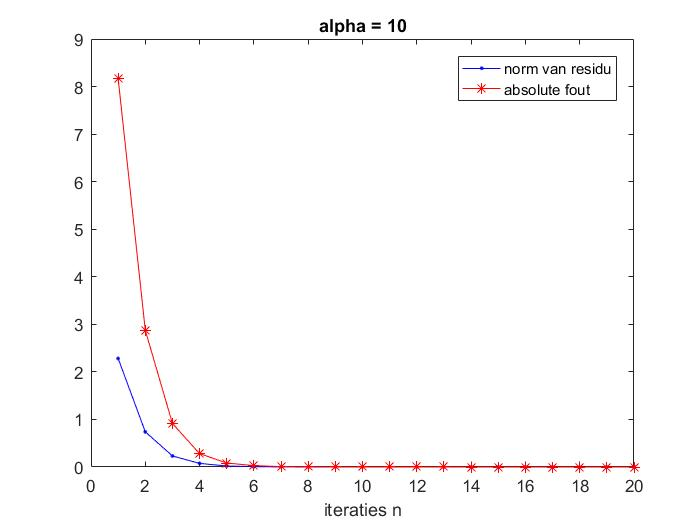
\includegraphics[width=\linewidth]{oef8_10.jpg}
        \caption{{\small alpha = 10}}    
            \label{fig:oef8_10}
        \end{subfigure}

        \hfill

        \begin{subfigure}[b]{0.475\textwidth}
            \centering 
            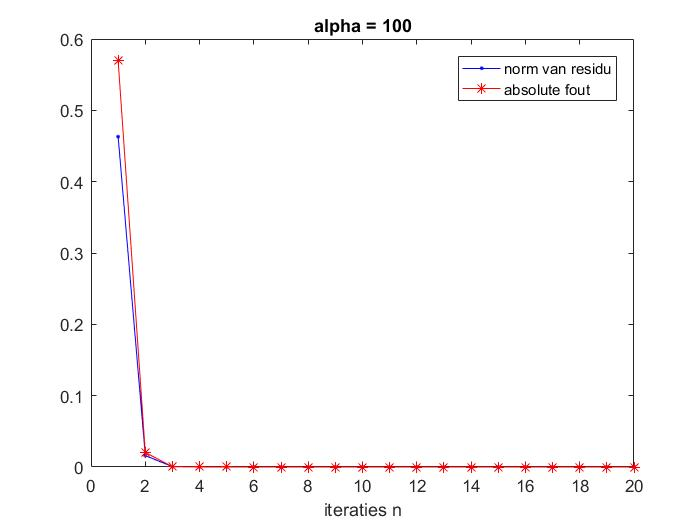
\includegraphics[width=\linewidth]{oef8_100}
            \caption{{\small alpha = 100}}
            \label{fig:oef8_100}
        \end{subfigure}

        \caption{convergentiegedrag voor verschillende waardes voor alpha} 
        \label{fig:oef8}
    \end{figure*}